\documentclass[12pt]{article}
\usepackage{graphicx}
\usepackage[letterpaper]{geometry}
\usepackage{times}
\geometry{top=1.0in, bottom=1.0in, left=1.0in, right=1.0in}

\usepackage{setspace}
\doublespacing

\usepackage{fancyhdr}
\pagestyle{fancy}

\lhead{}
\chead{}
\rhead{Petroff, Cao \thepage}
\lfoot{}
\cfoot{}
\rfoot{}
\renewcommand{\headrulewidth}{0pt}
\renewcommand{\footrulewidth}{0pt}

\setlength\headsep{0.333in}

\newcommand{\bibent}{\noindent \hangindent 40pt}
\newenvironment{workscited}{\newpage \begin{center} Works Cited \end{center}}{\newpage }

\begin{document}
\begin{flushleft}
Zachary Petroff, Kevin Cao \\
Professor Rodriguez \\
Introduction to Artificial Intelligence \\
5 May 2020

\begin{center}
Using the NEAT Algorithm to Teach Agents to Avoid Obstacles
\end{center}

\setlength{\parindent}{0.5in}
\noindent\textbf{Problem Space}

The game is fairly simple. The player controls a character that can only jump up, do a short hop, or move down. If the player is midair when moving down, the character accelerates quickly towards the ground. If the player is already on the ground, moving down allows the player to crouch.

Obstacles will begin moving toward the player at random intervals, and the player must evade the obstacles using either of the aforementioned movements. As the player passes each obstacle, the game gets progressively harder, and the obstacles begin moving faster and faster. Eventually, the obstacles are only on screen for a few frames, in which case it becomes near impossible for a human to evade the obstacles consistently.

To make the game slightly more difficult, there are a variety of obstacles. There are two types of ground obstacles, small and large. Small obstacles are shorter and narrower, and can spawn in groups of size 1 to 3. Large obstacles are taller and wider, and can spawn in groups of 1 to 4. Naturally, this makes large obstacles harder to navigate. To avoid these, the player must jump.

In addition, there are flying obstacles, which can spawn at three different elevations: ground, player level, or player jump level. Ground level flying obstacles must be jumped over. Player level flying obstacles spawn at around the same height as the top of the player. The player can still choose to jump over these, but the player can also crouch under them. The final elevation is the highest, and the obstacle spawns around the same level at which the player can jump to. That means that the player cannot jump over them, and any attempt to do so will result in a loss. Instead the player can choose to not move at all, or crouch.

Theoretically, the entire game could be beaten on the basis of pure simple calculation. Set some conditions to always crouch under flying obstacles. For other obstacles, calculate the distance to the obstacle and how long a jumping action takes. From there, it takes simple math to determine the correct jump timing. However, this went against the spirit of artificial intelligence, so we decided to take a more ``interesting" route by going with a genetic algorithm.

The genetic algorithm largely takes care of itself with regards to improving the agent. It is meant to emulate natural selection, so provided the correct environment, it would take care of the rest. For the programmers, the focus is on creating the optimal environment.

Therefore, the problem space focused primarily on input. What input should be provided to the agents? Too much data can result in slower evolution, as unnecessary mutations are wasted on irrelevant input. However, too little data would mean that the agents would not have sufficient data to actually beat the game.

\hfill

\noindent\textbf{Algorithms}

\noindent\textbf{Neuroevolution of Augmenting Topologies}

\noindent\emph{Explaining the Algorithm}

The Neuroevolution of Augmenting Topologies (NEAT) was used to create the neural network of the AI agents. In short, the algorithm works by initializing agents with a minimal neural network, an input layer, an output layer, and one connection between the two. The agents play the game, and their scores are recorded as their fitness level. To increase the complexity of these neural networks, new agents can be created from mutating old agents, or performing a crossover between two agents. There are three types of mutations:

\begin{enumerate}
  \item\textbf{Mutating Existing Connection:} an existing connection can be mutated so that its weight is changed. While it is likely that the weight is changed within a uniform pertubance, it can also be changed to be completely different from what it used to be.
  \item\textbf{Adding a New Connection:} a completely new connection can be made between two existing nodes, and it will be provided some random weight uniformly picked from a range of -1 to 1.
  \item\textbf{Adding a New Node:} a new node can be created such that it takes an old connection between existing nodes A and B, disables the connection, and creates a new connection from A to the new node with a weight of 1, and a new connection from the new node to B with the weight of the old connection. A single node in the neural network is a perceptron, that has a slightly modified sigmoid activation function.
\end{enumerate}

Each generation attempts the game, and weaker members are removed and stronger members are permitted to reproduce to build the next generation. We continue this selective removal until we find an agent that performs satisfactorily.

However, simply removing weaker players would also remove any valid attempts at mutation. While most mutations are bad, the trend towards beneficial behavior is often characterized by a series of individually harmful mutations. To protect these "innovative" mutations, the population is divided into species of similar agents (agents with a similar genome), and agents must only compete with members of their own species. With speciating, even if a particular agent does poorly compared to the entirety of the population, it can still be allowed to reproduce if it does well within its own species. This is key in allowing the population to produce an optimal agent. If a species does not improve after a set amount of generations, the species will then be deleted.

A question could be raised, ``how does one determine what species an agent belongs to?". To answer this, we have to introduce another key characteristic of the NEAT algorithm, innovation markers. Every new connection is provided a historic marking (typically a number), one that uniquely identifies it to the nodes it connects and the genome it first appeared in. From that point forward, all connections that match this connection are given the same number. This solves one of the main problems with crossover, competing conventions. By donig a standard crossover, we can lose important data. For example, performing a crossover between genes ABC and CBA (such that we crossover at each position, A does a crossover with C, B does a crossover with B, etc.), we could potentially result in ABA or CBC. In both instances, we have lost a node. NEAT avoids this problem by only performing a crossover on genes with a matching innovation marker. By doing so, we cannot potentially lose nodes because a connection is only crossed with a connection that connects the same two nodes.

By using these innovation markers, we can also compare two genomes to determine how ``similar" they are. When comparing two genomes, A and B, A is said to have an excess gene if it contains a innovation marker that B does not have. If B has an innovation marker that A does not have, then A is said to have a disjoint gene. By counting the number of disjoint genes and excess genes, multiplying by a constant, and then considering the average difference in weight between the matching genes of the two genomes, we can build a value that represents the differnece between the two genes. If the difference is below some threshold, then the two genomes are said to be in the same species.

\hfill

\noindent\emph{How the Neural Network Works}

There are three layers to the neural network, an input layer, hidden layer, and output layer. As mentioned previously, the algorithm starts off all agents with just two of these layers, the input and output layer. However, as more mutations occur and new nodes are added, the hidden layer grows. The agents reads in the input, provided by the programmer, and performs a feed-forward of the data through the neural network, sequentially passing through one layer at a time. The output layer in this game contains three nodes, representing crouching, hopping, and jumping. If no value in the three nodes reach a certain threshold, the agent does nothing. Otherwise, the agent takes the maximum of the three nodes and performs the corresponding action.

\hfill

\noindent\textbf{Drawing Parallels Between Computation and Brain}

\noindent\emph{The Similarities Between a Perceptron and a Biological Neuron}

Like a perceptron, a biological neuron has a threshold that fires if and only if that threshold is reached. However, in a neuron, the distance from the threshold is much more dynamic. For a perceptron, the distance is decided by the inputs, but in a neuron, there might be an influx of sodium, an outflux of potassium, or the firing of a presynaptic neuron that all influence whether an action potential is fired. While both a perceptron and a neuron act on the all-or-none principle, in a perceptron, the influences governing whether or not an action potential is reached are much more transparent. 

Moreover, in a perceptron, there are weights that can be thought of as a measure of synaptic strength between neurons. The synaptic strength between neurons refers how much a presynaptic neuron firing influences the membrane potential of a postsynaptic neuron. The greater the synaptic weight, the more likely the postsynaptic neuron will fire as a result of the presynaptic neuron firing. Just as, in a perceptron, the greater the weight between an input node and an output node, the greater effect the input will have in reaching the threshold. However, due to the method of training (a genetic algorithm), the synaptic weights are chosen randomly and allowed to continue on if they produce the desired behavior. While, between neurons, synaptic strength is increased by a process called long-term potentiation, that occurs if the pre- and postsynaptic neurons fire at the same time.

\hfill

\noindent\emph{The Similarities Between Softmax and Lateral Inhibition}

Lateral inhibition occurs when an activated neuron reduces the activity of its neighbors (Bailey). Similarly, if we look at each of the output nodes when using the softmax activation function as neurons, if one neuron fires, this means that the rest of the neurons are inhibited and unable to fire. However, there are differences between lateral inhibition and softmax. In lateral inhibition, the activation of neighboring neurons merely reduces activation, while softmax completely suppresses all other neurons. Furthermore, when using the softmax, all neurons besides the one being activated are suppressed, meaning there is no correlation between suppression and distance from the activated neuron like in lateral inhibition. 

\hfill

\hfill

\noindent\textbf{Empirical Analysis}

The NEAT algorithm worked spectacularly with the provided input of

\begin{itemize}
\item Distance from obstacle (inverted so that the value would be higher the closer the obstacle was)
\item Y position of the obstacle
\item Height of the obstacle
\item Width of the obstacle
\item Obstacle speed
\item Size of gap between next two obstacles
\item Whether or not the obstacle was flying
\item Y position of the player
\end{itemize}

. In the first few generations, the agents would act randomly, only picking one of the four possible actions and repeating those actions. Typically, the top performing agents in the generation would learn to wait to jump until the obstacles got closer at around generation 7. This tactic would work well, except they would consistently fail the highest elevation flying obstacle, which could not be jumped over. It usually wouldn't be until generation 30 or so that the agents would learn to duck under flying obstacles instead of attempting to jump over them.

However, this second milestone would vary greatly depending on the challenges the agents faced. The obstacles were spawned randomly each generation, so if the population did not encounter high flying obstacles earlier, then it would take longer for the agents to learn to duck underneath them. This could be attributed to the fact that in most cases, the early form of a genotype that would duck underneath a flying obstacle would also attempt to duck underneath a grounded obstacle, which resulted in lower fitness for these species. However, due to speciation, these agents were still protected and allowed to reproduce, albeit at a much slower rate. Consequently, they would simply need to wait until a more suitable environment for them was created. If a high flying obstacle was spawned early within the first two obstacles, such that agents that did not crouch lost early, then there would be a much higher selective pressure to reproduce agents that did crouch. In some cases, we would see that the agents did not learn to crouch until generation 40.

From there, it was simply a measure of which agents would learn to time their jumps in accordance to the speed at which the obstacles were traveling. It would usually take till generation 55 before seeing a ``perfect" agent (one that could handle the game at peak difficulty without error), although this would rely heavily on when the agents reached the second milestone. In some of the more extreme cases, we saw agents reaching the second milestone at generation 15, and reaching perfection at generation 26. It became blatantly obvious that the environment the agents were more than significant factors in their growth.

\hfill

\noindent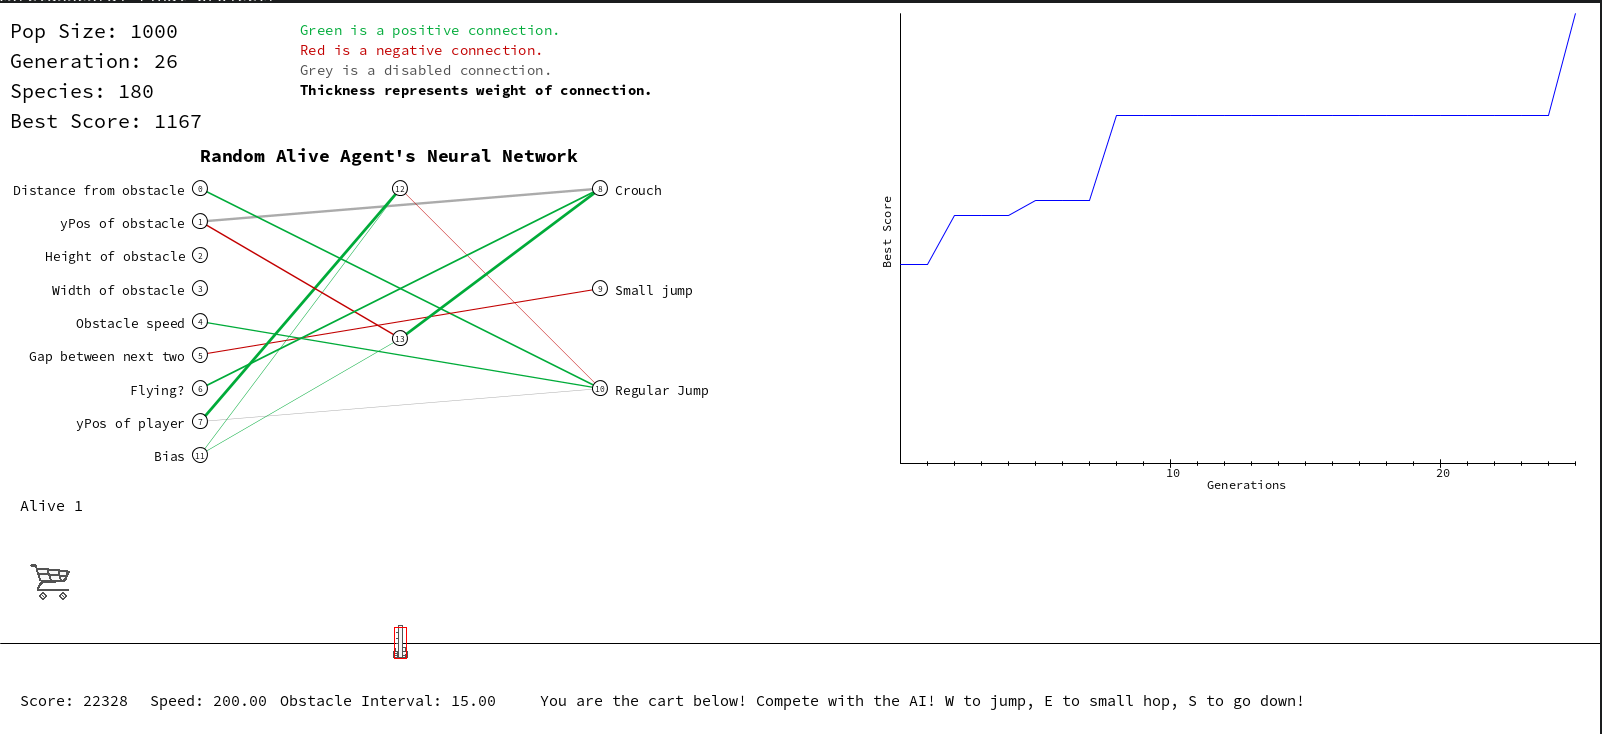
\includegraphics[scale=.4]{early_perfect.png}

The agents reached milestone 1 at generation 2, milestone 2 at generation 9, and hit perfect at generation 26.

\noindent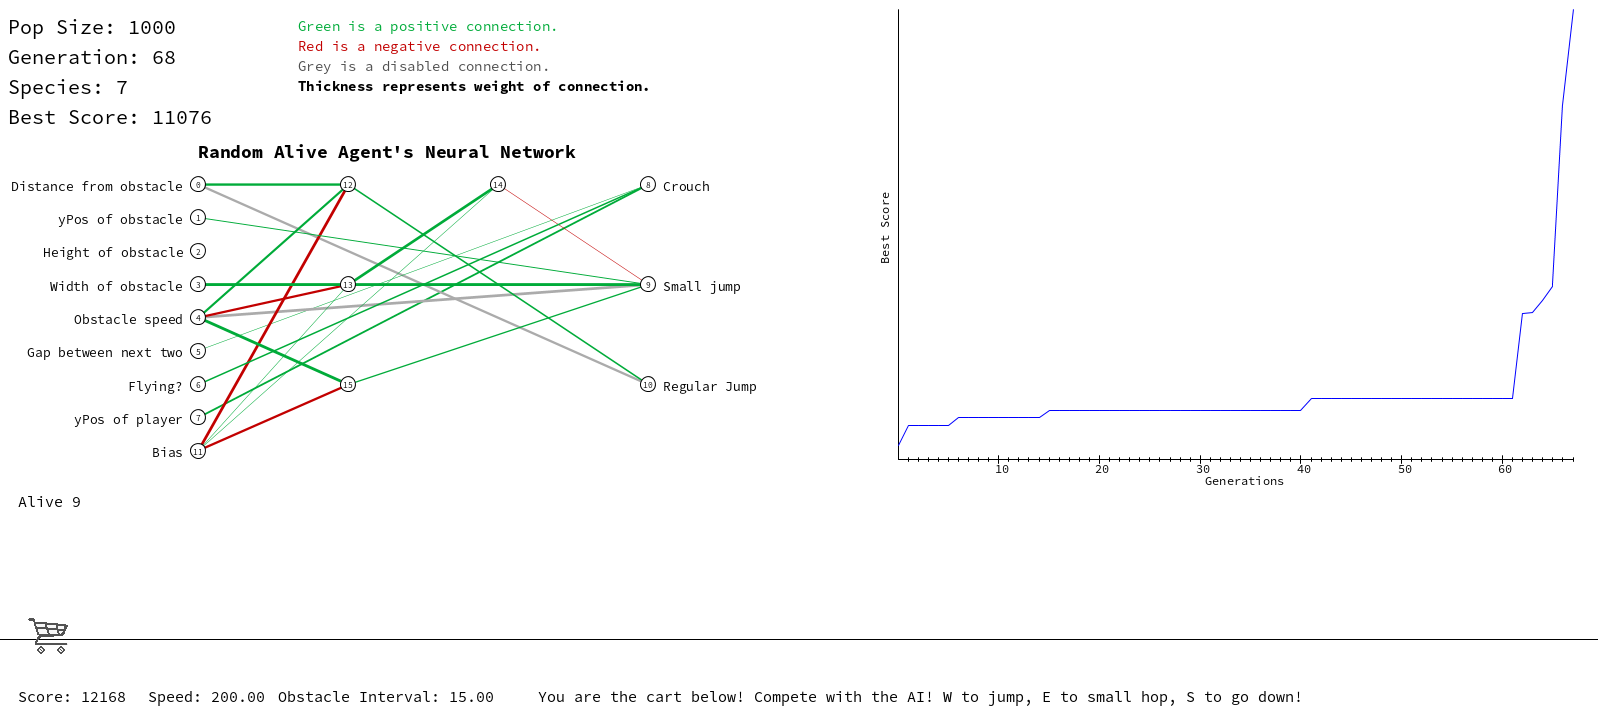
\includegraphics[scale=.4]{late_perfect.png}

The agents reached milestone 1 at generation 1, milestone 2 at generation 41, and hit perfection at generation 68. Was not until generation 40 that they were given a series of high flying obstacles.

\hfill

It is also important to node the input we provided the agents. Originally, agents were not provided the ``Flying?" input, and were only given the Y position of the obstacle. Interestingly enough, this resulted in significantly slower growth. In our testing, agents would not consistently duck underneath flying obstacles until generation 60, or in one extreme case, generation 94. And even then, they would not be reliable enough to even get close to a ``perfect" agent. It would not be until 126 before a perfect player was created. This was surprising, as the lowest flying obstacle had a Y position of 0, and all other flying obstacles had a positive Y position. It would be reasonable to assume that the agents would be able to differentiate between these values nearly as easily as they would the binary "Flying?" input.

\hfill

\noindent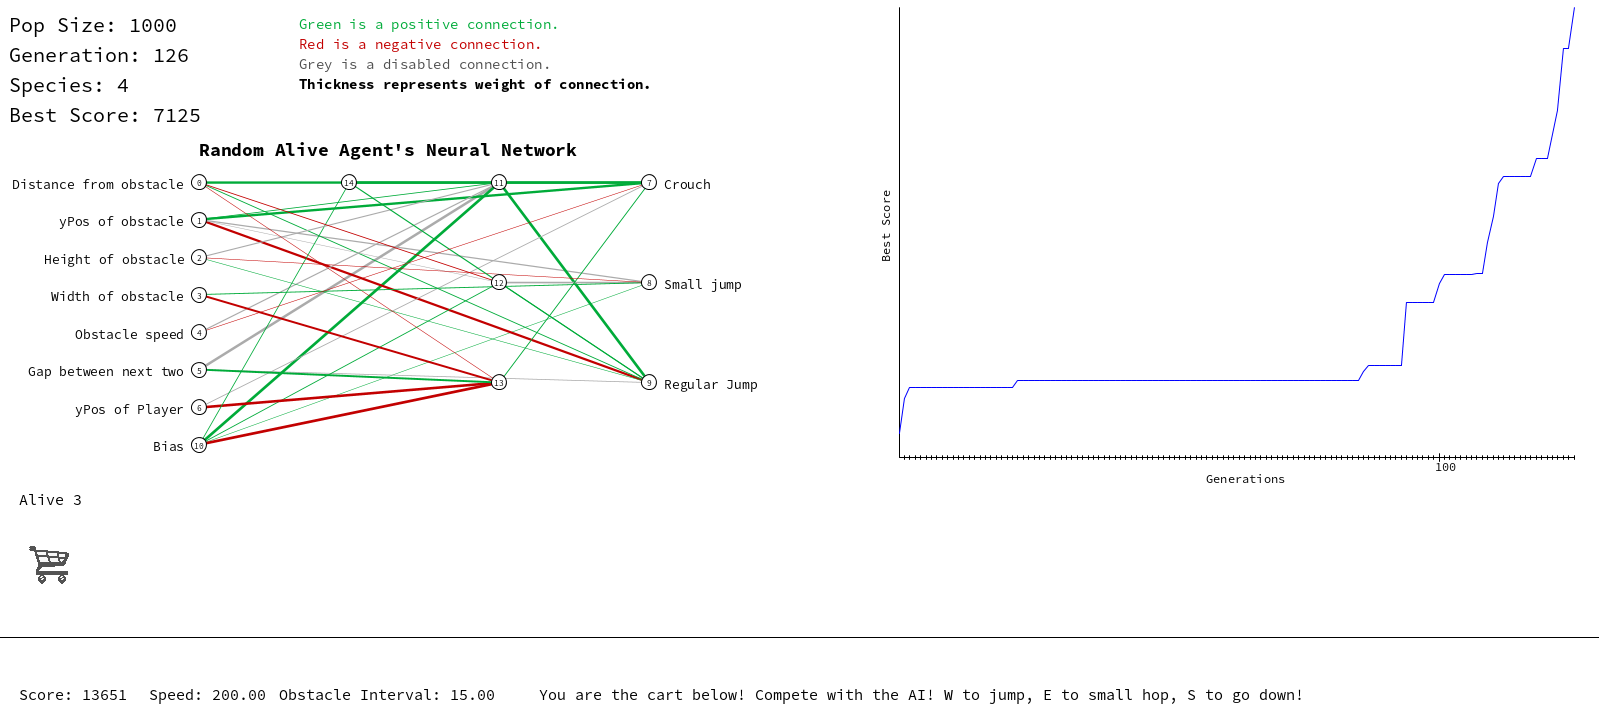
\includegraphics[scale=.4]{no_flying_bit.png}
The agents were not provided a flying bit, and growth was much slower. The agents reached milestone 1 at the same time, but did not reach milestone 2 until generation 94. Then the perfect player was reached much later after that, at generation 126.

\hfill

\noindent\textbf{Ways to Improve Performance}

\noindent\emph{Better Time Complexity Optimization}

The source code for the NEAT algorithm could certainly use improvement by optimizing certain methods. For example, when performing a crossover, a mapping from the parents' node to a duplicate node created for the child is created, increasing the space complexity for the crossover method. There certainly is a better way of going about it, but was not implemented due to time constraints. In addition, when calculating an innovation number for a new connection, we must search through all existing innovation numbers to determine that a number for the connection has not already been created, which is done in linear time. Perhaps with another code structure, this could be reduced to amortized constant time using hashing. In general, the code itself could certainly use refactoring, as a lot of changes were made without considering time complexity and only focusing on getting the algorithm to work.


\hfill

\noindent\emph{A Better Training Method}

Because genetic algorithms are subject to randomness, an improvement would be a more precise method of training. There exist many different methods, however, reinforcement learning seems to be the most effective when trying to teach a network how to play a game. There are many famous examples in the history of Artificial Intelligence that display the proficiency of reinforcement networks, such as DeepBlue and AlphaGo. 
Reinforcement networks learn by providing the player with a reward or punishment corresponding to each of its actions. With each iteration, the player is enticed to produce good behavior, while at the same time being cattle-prodded away from undesired behavior. This proves to produce unmatched results, and is more precise than the guess-and-check method used by a genetic algorithm. To explain exactly why this is desirable, consider the problem of trying to train an agent to navigate to the top of a mountain. A genetic algorithm might get lucky and produce an outcome that allows the agent to get very close to the top. However, the time it would take to find a better outcome is completely unknown. The genetic algorithm might explore thousands of worse solutions before it finds a better one. With reinforcement learning, on the other hand, the network could incrementally find better solutions, until it reaches the top. In other words, we know roughly how long the training would have to take place and how well our network could do. 

\hfill

\noindent\textbf{Acknowledgements}

In implementing this algorithm, the original research paper was referenced heavily, and can be found in the works cited in the next page. In addition, to understand how the algorithm worked, Hydrozoa's videos on implementing his HydroNEAT algorithm were incredibly useful in transforming the technical explanation of the paper to actual implementation. Lastly, CodeBullet's implementation of the NEAT algorithm was useful in demonstrating a more digestable, simpler method of integrating the algorithm with a game. In addition, the visualization of the neural network was largely created by CodeBullet, with slight modifications made to optimize the visualization. All of these sources can be found below.

\begin{workscited}
\thispagestyle{plain}
\bibent
  Bailey, Regina. “Lateral Inhibition: Neuron Suppression Enhances Sensory Perception.” \emph{ThoughtCo}, ThoughtCo, 30 June 2019, www.thoughtco.com/lateral-inhibition-4687368.

\bibent
  CodeBullet. ``AI learns to play Google Chrome Dinosaur Game || Can you beat it??." \emph{YouTube}, uploaded by CodeBullet, 29th April 2018, www.youtube.com/watch?v=sB\_IGstiWlc.

\bibent
  Hydrozoa. ``Implementing NEAT algorithm in java." \emph{YouTube}, uploaded by Hydroazoa, 18th Jan. 2018, www.youtube.com/watch?v=1I1eG-WLLrY.

\bibent
  Stanley, Kenneth O., and Risto Miikkulainen. “Evolving Neural Networks through Augmenting Topologies.” Evolutionary Computation, vol. 10, no. 2, 2002, pp. 99–127.
\end{workscited}
\end{flushleft}
\end{document}
